% ClearEval MICCAI 2026 main conference submission (LNCS format)
% This file is designed to compile out-of-the-box on Overleaf.
% It follows the provided "MICCAI2026-main conference paper template.tex".

\documentclass[runningheads]{llncs}

\usepackage[T1]{fontenc}
\usepackage{graphicx,verbatim}
\usepackage{amsmath,amssymb}
\usepackage{booktabs}
\usepackage{multirow}
\usepackage{url}

\begin{document}

\title{ClearEval: A Data-driven Benchmark for
Evaluating Large Language Models in Tissue Optical Clearing}
\titlerunning{ClearEval:A Data-driven Benchmark for TOC}
%\titlerunning{ClearEval}

\begin{comment}  %% Removed for anonymized MICCAI submission
\author{First Author\inst{1}\orcidID{0000-1111-2222-3333} \and
Second Author\inst{2,3}\orcidID{1111-2222-3333-4444} \and
Third Author\inst{3}\orcidID{2222--3333-4444-5555}}
\authorrunning{F. Author et al.}
\institute{University A \and University B \email{author@institute.edu}}
\end{comment}

% NOTE: Do not remove this anonymized author section for initial submission.
\author{Anonymized Authors}
\authorrunning{Anonymized Author et al.}
\institute{Anonymized Affiliations \\
    \email{email@anonymized.com}}

\maketitle

\begin{abstract}
Tissue Optical Clearing (TOC) enables high-resolution 3D visualization, yet complex protocol design risks irreversible specimen damage. While LLMs excel at knowledge retrieval, their ability to synthesize viable wet-lab protocols remains under-evaluated. We introduce ClearEval, the first expert-curated benchmark for TOC protocol design. Moving beyond semantic similarity, we evaluate 13 SOTA LLMs via a dual-track pipeline: static knowledge is assessed via MCQs, while practical generation is evaluated through our novel Completeness, Correctness, and Effectiveness (CCE) framework. CCE serves as an empirically grounded, text-reference-free metric, assessing viability through formulas derived from experimental confidence intervals rather than static texts. Results show that while models exceed 80\% accuracy in static retrieval, performance drops significantly for executable protocols. Challenges in incubation time estimation and chemical incompatibility expose a critical “knowledge-execution gap” in scientific AI. This strategy provides a robust validation framework for future scientific agents. The dataset and code are publicly available at https://github.com/404NotFound422/ClearEval-public.

\keywords{Benchmark \and Tissue optical clearing \and Wet-lab protocols \and Large language models  }
\end{abstract}

\section{Introduction}
Tissue Optical Clearing (TOC) homogenizes refractive indices to enable non-destructive, sub-cellular 3D imaging via light-sheet microscopy~\cite{ueda2020tissue,chung2013clarity}, preserving long-range connectivity essential for high-fidelity organ atlases~\cite{wang2025advances,richardson2025unlocking}. However, TOC protocol design is a complex multi-objective optimization problem where parameter misjudgments risk irreversible specimen damage, making traditional trial-and-error approaches both costly and inefficient.

While LLMs demonstrate proficiency in biomedical question answering~\cite{singhal2023medpalm}, existing scientific benchmarks (e.g., MedQA~\cite{jin2021disease}, MMLU~\cite{hendrycks2021mmlu}) and their recent extensions~\cite{zhang2025benchmarking,wang2025cardbiomedbench,feng2024mediq} predominantly assess static knowledge recall without grounding in experimental validation. Furthermore, traditional semantic metrics like BLEU~\cite{papineni2002bleu} and general-purpose evaluators~\cite{liu2023geval,li2024survey} fail to capture functional executability. Linguistically fluent protocols can remain experimentally invalid due to incorrect concentrations or processing times—subtle wet-lab errors that generic evaluators often overlook, thereby propagating hallucinations~\cite{bang2025hallulens,zhang2025survey}. Evaluating scientific LLMs thus requires a paradigm shift: from text-based similarity to rigorous protocol validation driven by empirical evidence.

To bridge this gap, we introduce \textbf{ClearEval}, a benchmark for wet-lab grounded TOC protocol design that integrates an evaluation pipeline constructed from extensive experimental data. We propose the \textbf{CCE (Completeness, Correctness, Effectiveness) framework}, which quantitatively validates protocol executability against empirical confidence intervals. Our main contributions are: (1) a novel benchmark paradigm for evaluating the functional executability of LLM-generated protocols; (2) a curated dataset comprising 2,589 domain-specific MCQs and 253 experiment-driven tasks; and (3) the data-driven CCE framework that leverages formulaic assessment to measure LLM performance gaps in practical planning.

\section{Related Works}
Scientific LLM evaluation has largely focused on static knowledge retrieval~\cite{hendrycks2021mmlu,jin2021disease,singhal2023medpalm} or multidimensional reasoning via frameworks like SeedBench~\cite{ying2025seedbench}. While recent advances~\cite{martinez2025ai,gupta2025wetbench} highlight the need to bridge computational predictions and experimental validation, existing metrics like BLEU~\cite{papineni2002bleu} and G-Eval~\cite{liu2023geval} may not fully capture functional executability. This discrepancy often allows linguistically coherent but experimentally invalid protocols to remain undetected, potentially masking hallucinations~\cite{bang2025hallulens} regarding chemical compatibility or incubation requirements. Unlike text-centric approaches, ClearEval proposes a text-reference-free paradigm grounded in the empirical parameters of Tissue Optical Clearing~\cite{ueda2020tissue,chung2013clarity,kumar2024tissue}.

\section{The ClearEval Benchmark}
The development of ClearEval follows a structured pipeline that transforms specialized TOC domain expertise into a computational evaluation framework (Fig.~\ref{fig:overview}). 

\begin{figure}
    \centering
    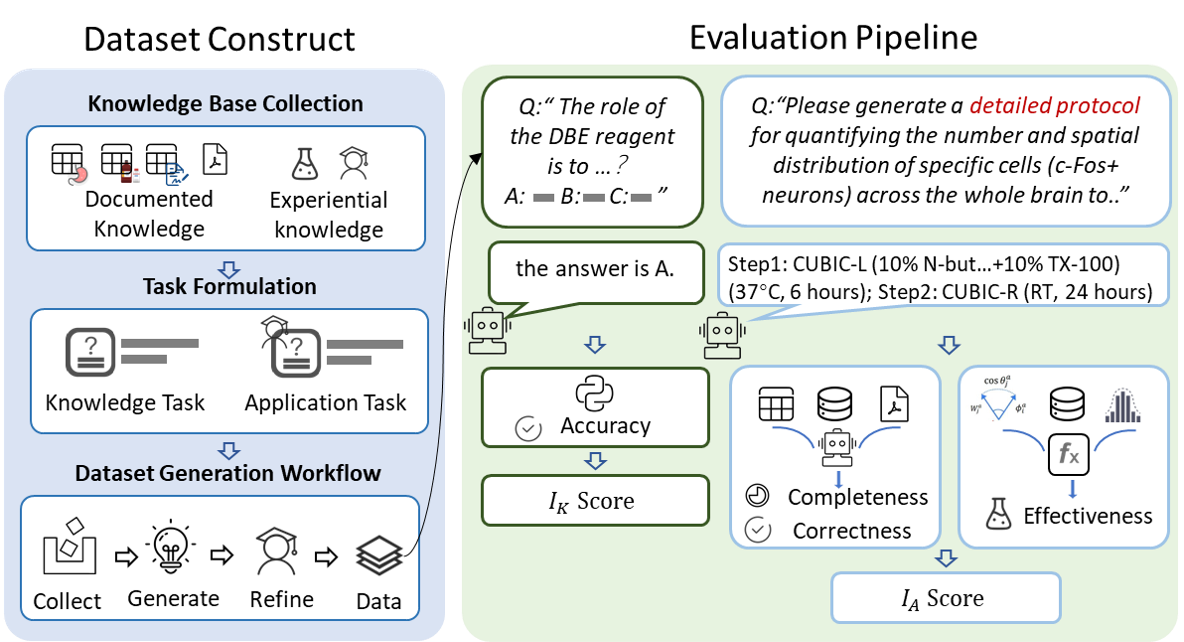
\includegraphics[width=1\linewidth]{figures/overview.png}
    \caption{Overview of the dataset construction and benchmarking pipeline. The left panel shows the workflow for formulating domain knowledge into evaluation datasets. The right panel details the evaluation process, scoring knowledge tasks on accuracy ($I_K$) and application tasks on completeness, correctness, and a data-driven effectiveness metric ($f_x$) grounded in experimental confidence intervals to calculate the $I_A$ Score.}
    \label{fig:overview}
\end{figure}

\subsection{Knowledge Base and Task Formulation}
ClearEval formalizes wet-lab constraints into a structured knowledge system by integrating curated metadata on tissue types, molecular markers, and physicochemical properties from over 30 mainstream TOC articles.To align user requirements with protocol selection, these constraints are mapped into a 6-dimensional vector space $\mathcal{V} \in[0,1]^6$ representing key performance indicators such as fluorescence preservation, reagent permeability, and biosafety. Within this space, 60 core scientific missions across various biological scales were defined by experts to serve as seeds for realistic task generation.

\subsection{Dataset Generation Workflow}
The ClearEval pipeline (Fig.~\ref{fig:overview}, bottom left) utilizes a DeepSeek-driven RAG system to synthesize task candidates from 70 decision templates, 60 mission seeds, and 437 literature-derived data chunks. Each candidate underwent rigorous expert validation to ensure scientific integrity and eliminate hallucinations. The resulting dataset comprises \textbf{2,589 Knowledge Tasks (MCQs)} featuring an 8-option format to minimize the probability of correct guessing, and \textbf{253 Application Tasks (OEQs)}. Notably, the OEQs move beyond static reference texts, utilizing instead a series of constrained scenarios evaluated through an automated, experiment-based scoring pipeline (Fig.~\ref{fig:overview}, right).

\section{Evaluation Framework}
To quantify the transition from theoretical recall to functional executability, ClearEval employs a hierarchical scoring system (Table~\ref{tab:metrics}). The Application Index ($I_A$) shifts the focus from semantic similarity to \textbf{empirically grounded verification}, utilizing experimental confidence intervals to evaluate the viability of generated protocols.

\begin{table}[htbp]
    \centering
    \caption{The Hierarchical Metric System of ClearEval. Evaluation scales from static knowledge retrieval to empirically-grounded protocol execution.}
    \label{tab:metrics}
    \resizebox{\textwidth}{!}{
    \begin{tabular}{l l l l c} 
        \toprule
        \textbf{Level} & \textbf{Dimension} & \textbf{Sub-Metric} & \textbf{Method} & \textbf{Max} \\
        \midrule
        Knowledge ($I_K$) & Static Retrieval & Accuracy & Deterministic & 100\% \\
        \midrule
        \multirow{9}{*}{Application ($I_A$)} & \multirow{2}{*}{Completeness} & Step Integrity & LLM-Judge & 40\% \\
         & & Param Detail & LLM-Judge & 60\% \\
        \cmidrule{2-5} 
         & \multirow{3}{*}{Correctness} & Sequential Logic & LLM-Judge & 40\% \\
         & & Consistency & LLM-Judge & 20\% \\
         & & Physics Plausibility & LLM-Judge & 40\% \\
        \cmidrule{2-5} 
         & \multirow{4}{*}{Effectiveness} & Method Suitability & Vector Sim. & 30\% \\
         & & Label Compatibility & Rule-Based & 40\% \\
         & & Trans. Validity ($S_{trans}$) & Physics Eq. & 15\% \\
         & & Time Efficiency ($S_{time}$) & Physics Eq. & 15\% \\
        \midrule
        \textbf{Overall} & Expert Score & Harmonic Mean & Aggregation & 100\% \\
        \bottomrule
    \end{tabular}%
    }
\end{table}

\subsection{Knowledge ($I_K$) and Application ($I_A$) Indices}The \textbf{Knowledge Index ($I_K$)} represents the macro-averaged MCQ accuracy across domain-specific categories. To evaluate protocol design, the \textbf{Application Index ($I_A$)} adopts a bottleneck formulation:
\begin{equation}
I_A = \min(\text{Completeness}, \text{Correctness}, 
\text{Effectiveness})
\end{equation}
This "weakest-link" approach reflects wet-lab realities, where a single critical failure in logic or chemical compatibility can render an entire experiment invalid.

\subsection{Empirically-Grounded Effectiveness ($E_{score}$)}
This dimension quantitatively verifies protocol feasibility against expert databases and physical constraints, yielding $E_{score} = S_{method} + S_{label} + S_{trans} + S_{time}$:

\noindent\textbf{1. Method \& Label Suitability:} 
$S_{method}$ evaluates the cosine similarity between the generated and expert constraint vectors: 
\begin{equation}
S_{method} = 5 \times \text{ReLU}(\cos(\mathbf{v}_{pred}, \mathbf{v}_{ref})). 
\end{equation}
$S_{label}$ is a \textbf{hard constraint}, scoring 0 if any fluorescence quenching risk is detected.

\noindent\textbf{2. Transparency ($S_{trans}$) \& Time Efficiency ($S_{time}$):} 
To evaluate continuous parameters against \textbf{experimental confidence intervals}, we penalize Refractive Index (RI) mismatches and incubation time deviations ($\Delta t$) using Gaussian functions:
\begin{equation}
S_{trans} = 3 \cdot \exp \left( - \frac{(RI_{pred} - RI_{ref})^2}{2\sigma_{RI}^2} \right), \quad
S_{time} = 3 \cdot \exp \left( - \frac{\Delta t^2}{2\tau^2} \right)
\end{equation}
where $\sigma_{RI}$ and $\tau$ are expert-defined tolerance parameters. For $S_{time}$, $\Delta t$ measures the deviation from the physically viable time window $[t_{min}, t_{max}]$.
The raw $E_{score}$, which aggregates the Empirically-Grounded equations to a theoretical maximum of 17 points, is subsequently min-max normalized to a $[0, 100]$ scale. This aligns it with the Completeness and Correctness dimensions before computing the final $I_A$ bottleneck.

\subsection{Overall Expert Score}
To penalize models that memorize facts but fail under practical physical constraints, the \textbf{ClearEval Expert Score} is the harmonic mean: $\text{Score} = 2 I_K I_A / (I_K + I_A)$. Given the bottleneck formulation of $I_A$, a high score demands both broad theoretical recall and strict experimental compliance.

\section{Experiments}
\subsection{Models and Settings}
We benchmarked LLMs across the GPT, Gemini, Claude, DeepSeek, and Qwen families. We set the temperature to $0.0$ for \textbf{Knowledge tasks} to ensure reproducibility, and used official default temperatures for \textbf{Application tasks} to enable reasoning models to fully explore Chain-of-Thought (CoT).

\subsection{Main Results: The Knowledge-Execution Gap}
Table~\ref{tab:main_results_total} reveals a stark capability imbalance between static recall and wet-lab execution. This is visually highlighted in Fig.~\ref{fig:radar_chart}: the left panel demonstrates that all evaluated models exhibit uniformly high and tightly clustered proficiency across Knowledge dimensions. In stark contrast, Application Performance (right) is highly erratic. While models generally maintain basic procedural completeness, their trajectories scatter unpredictably and collapse sharply on Effectiveness metrics (e.g., exact RI matching, viable diffusion times), exposing a severe knowledge--execution gap.

\begin{table}[htbp]
    \centering
    \caption{Performance of state-of-the-art models on ClearEval. Evaluation covers Knowledge (MCQ) and Application (OEQ). $I_K$ represents the average of the Knowledge subset, $I_A$ represents the minimum score across the Application subset, and Total is their harmonic mean.}
    \label{tab:main_results_total}
    
    % 微调列间距以防缩放过度
    \setlength{\tabcolsep}{3pt} 
    
    % 使用 resizebox 强制表格宽度自适应当前版面宽度
    \resizebox{\textwidth}{!}{%
    \begin{tabular}{l cccc cccc c} 
        \toprule
        \multirow{2}{*}{\textbf{Models}} & \multicolumn{4}{c}{\textbf{Knowledge (MCQ)}} & \multicolumn{4}{c}{\textbf{Application (OEQ)}} & \multirow{2}{*}{\textbf{Total}} \\
        \cmidrule(lr){2-5} \cmidrule(lr){6-9} 
        & Tissue & Reagent & Method & $I_K$ & Com. & Cor. & Eff. & $I_A$ & \\
        \midrule
        
        \multicolumn{10}{l}{\textit{Proprietary Models}} \\
        \midrule
        GPT-5.2-Fast & \textbf{91.1} & \textbf{88.7} & 93.5 & \textbf{91.1} & \underline{87.1} & \textbf{90.2} & 66.4 & 66.4 & \textbf{76.8} \\
        GPT-5.2-Think & \underline{90.5} & \underline{87.3} & \underline{93.6} & \underline{90.5} & 80.4 & 88.3 & 64.1 & 64.1 & 75.0 \\
        Gemini-3-Flash & 78.7 & 81.8 & 91.1 & 83.9 & 84.6 & 83.3 & 66.4 & 66.4 & 74.1 \\
        Gemini-3-Pro & 88.8 & 77.2 & 86.7 & 84.2 & 81.7 & 84.8 & 66.3 & 66.3 & 74.2 \\
        Claude-4.6-Sonnet & 87.6 & 82.9 & \textbf{94.9} & 88.5 & \textbf{100.0} & 85.8 & 54.2 & 54.2 & 67.2 \\
        
        \midrule
        \multicolumn{10}{l}{\textit{Open-Weight Models}} \\
        \midrule
        GLM-4.7 & 79.3 & 80.2 & 93.5 & 84.3 & 81.9 & \underline{89.6} & \underline{69.0} & \underline{69.0} & 75.9 \\
        GLM-4.7-Think & 78.7 & 70.5 & 90.7 & 80.0 & 78.8 & 87.1 & \textbf{70.3} & \textbf{70.3} & 74.8 \\
        DeepSeek-V3.2 & 79.9 & 77.9 & 91.7 & 83.2 & 84.6 & 76.2 & 62.2 & 62.2 & 71.2 \\
        DeepSeek-V3.2-Think & 85.3 & 83.8 & 93.5 & 87.5 & 75.0 & 71.9 & 62.3 & 62.3 & 72.8 \\
        Qwen3-max & 79.9 & \underline{87.3} & 93.1 & 86.8 & \underline{87.1} & 81.0 & 68.1 & 68.1 & \underline{76.3} \\
        Qwen3-235B-A22B & 77.5 & 81.2 & 89.1 & 82.6 & 64.6 & 67.1 & 53.9 & 53.9 & 65.2 \\
        Qwen3-32B & 73.4 & 78.6 & 89.9 & 80.6 & 56.2 & 46.5 & 55.2 & 46.5 & 59.0 \\
        Qwen3-14B & 73.4 & 77.8 & 88.4 & 79.9 & 48.8 & 39.0 & 54.3 & 39.0 & 52.4 \\

        \bottomrule
    \end{tabular}%
    }
\end{table}

\begin{figure}[htbp]
    \centering
    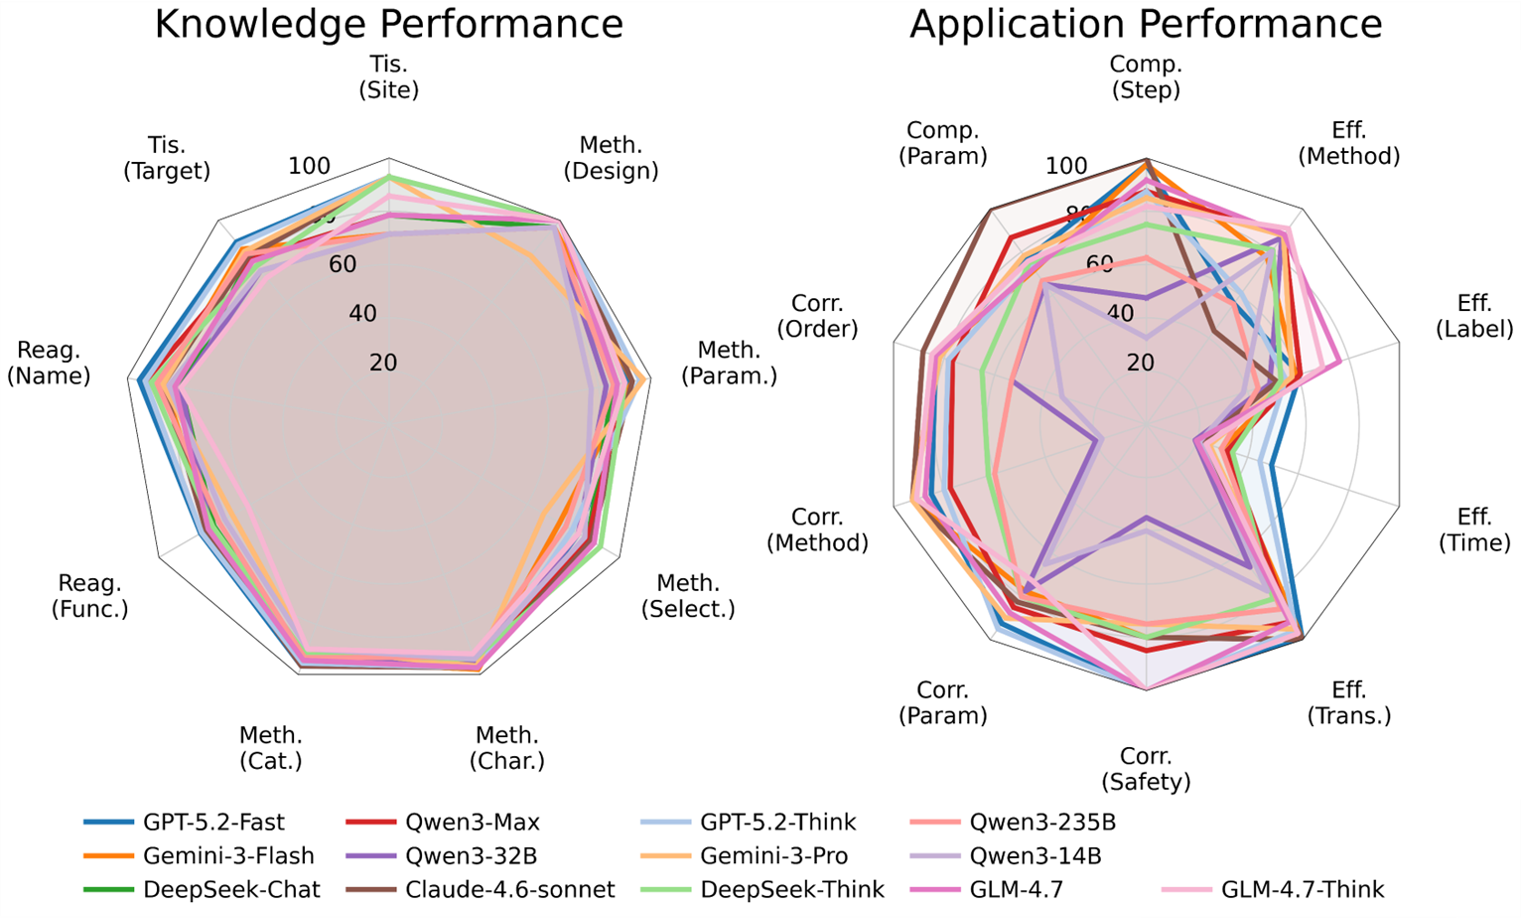
\includegraphics[width=1\linewidth]{figures/combined_radar_chart (6).png}
    \caption{Performance comparison of 13 LLMs on the ClearEval benchmark. The left panel shows Knowledge Performance ($I_K$) across domain-specific attributes (Tissue, Reagent, Method). The right panel details Application Performance ($I_A$), evaluated on completeness, correctness, and a Empirically-Grounded effectiveness metric.}
    \label{fig:radar_chart}
\end{figure}

\subsection{Human Alignment of the Automated Metrics}
We validated our automated evaluation pipeline against blinded expert judgments on a subset of 260 generated protocols. As shown in Fig.~\ref{fig:alignment}a, alignment varies depending on the underlying evaluation mechanism. Dimensions relying on generic LLM-as-a-judge (Completeness and Correctness) exhibit moderate-to-strong correlations (Pearson $r=0.77$ and $0.69$, respectively), reflecting the inherent instability of LLMs in assessing complex wet-lab logic. Crucially, our core proposed dimension—the Empirically-Grounded Effectiveness—achieves a strong correlation ($r=0.83$), demonstrating that mathematical constraints provide a far more reliable proxy for expert judgment. 

\begin{figure}[htbp]
    \centering
    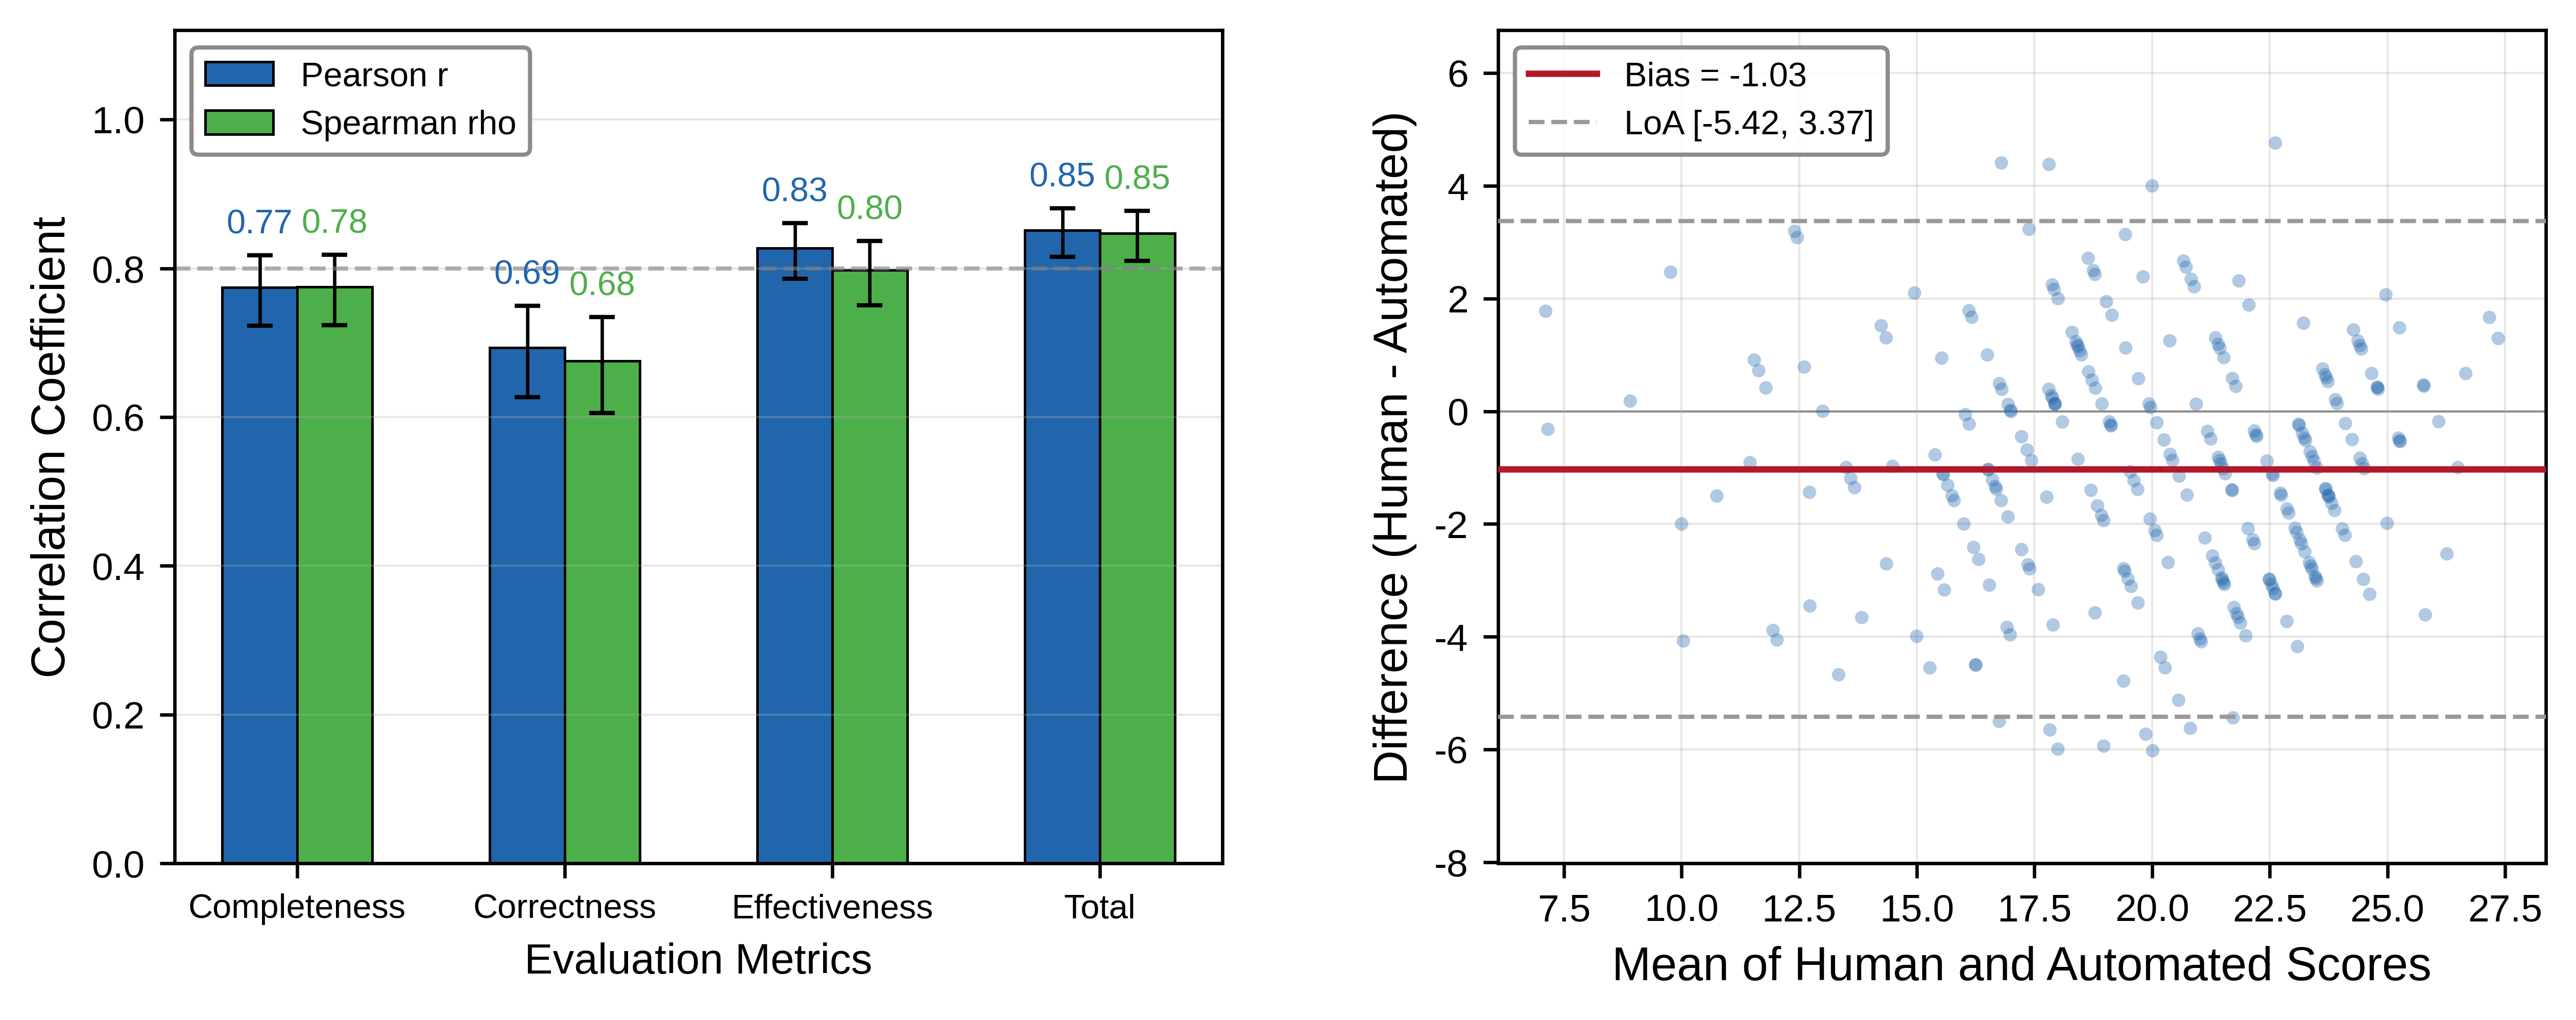
\includegraphics[width=1\linewidth]{figures/conbined_alignment_plots(7).png}
    \caption{Human alignment of automated metrics. (a) ClearEval metrics show strong correlation with expert ratings.(b) Bland-Altman plot reveals high absolute agreement with a minimal bias of -1.03.}
    \label{fig:alignment}
\end{figure}

\subsection{Fine-Grained Diagnosis: Effectiveness Bottlenecks}Analysis of specific failure modes (Fig.~\ref{fig:violin_limits}) reveals that the Effectiveness bottleneck is primarily driven by Time Efficiency ($S_{time}$) and Label Compatibility ($S_{label}$).In \textbf{Time Efficiency} ($S_{time}$), models exhibit significant \textit{scale-insensitivity}. While ground-truth missions span a 0--200 hour window, generated durations occasionally reach 800 hours. This reflects a systematic bias: LLMs tend to underestimate incubation requirements for large intact tissues while overestimating those for thin sections.Regarding \textbf{Label Compatibility} ($S_{label}$), the broad score distributions indicate inconsistent performance across chemical contexts. While models successfully recall high-frequency knowledge—such as protein quenching by organic solvents—they struggle to manage complex compatibilities between diverse synthetic dyes and specific TOC methodologies. 

\begin{figure}[htbp]
    \centering
    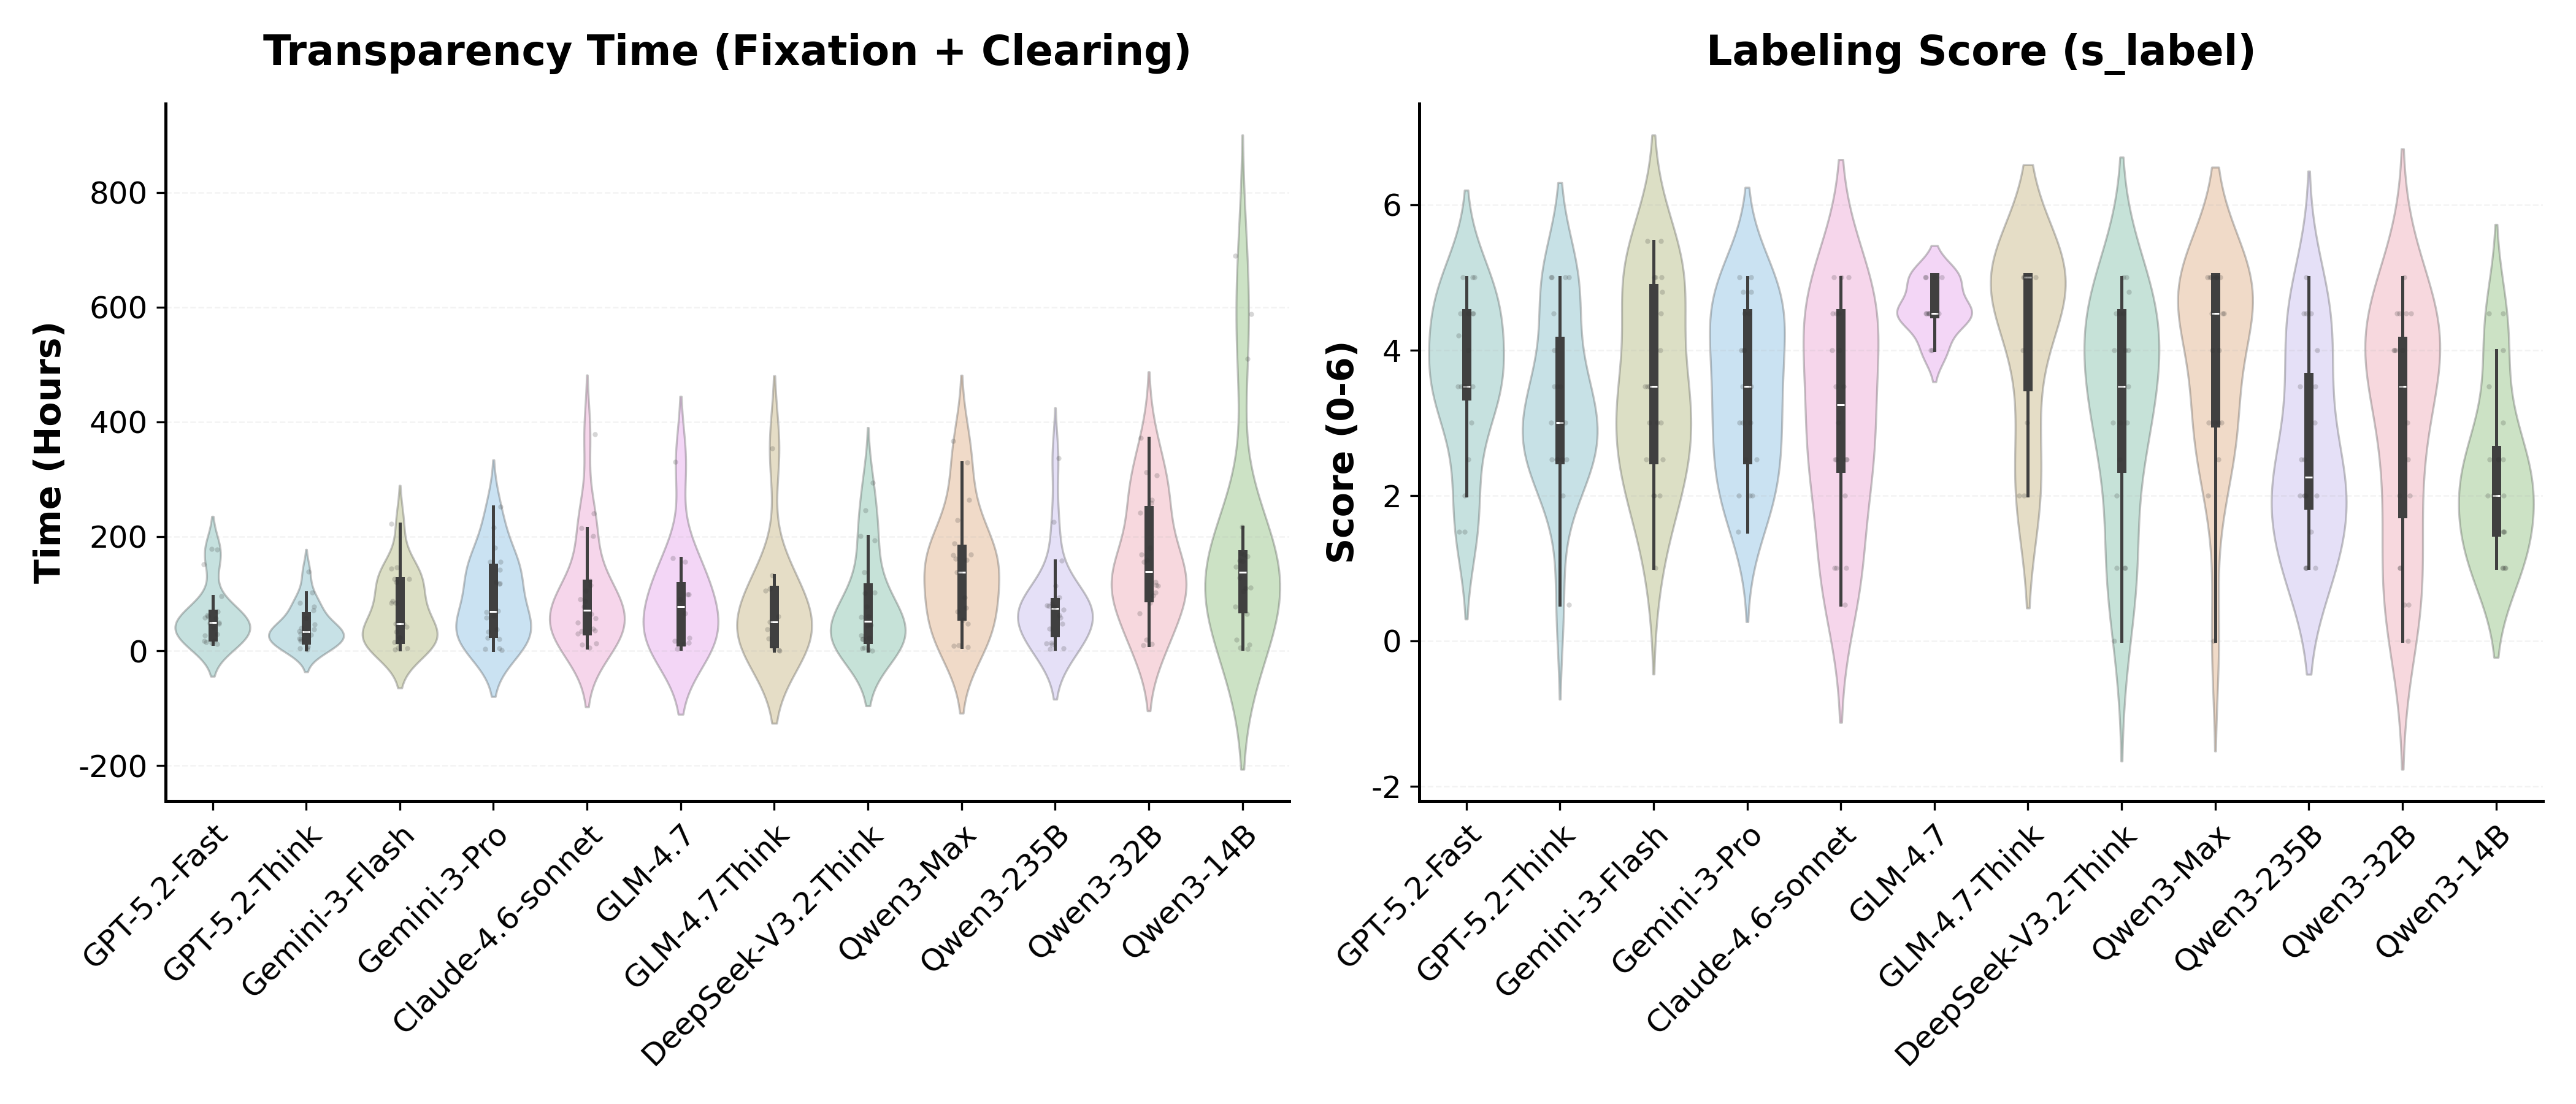
\includegraphics[width=1\linewidth]{figures/combined_violin_plots.png}
    \caption{Performance distributions of LLMs regarding transparency time estimation and labeling compatibility.}
    \label{fig:violin_limits}
\end{figure}

\section{Discussion and Limitations}
ClearEval demonstrates that the primary bottleneck in scientific AI is not declarative knowledge retrieval, but the absence of empirical grounding. This knowledge-execution gap suggests that for LLMs to become viable in specialized domains, they must transition into grounded scientific agents that internalize experimental constraints—such as reagent diffusion scales—within their reasoning loops. Such agents could serve as the decision-making core for automated laboratory instruments, ensuring protocols are functionally executable rather than merely linguistically plausible.

However, ClearEval remains a static paradigm. Real-world wet labs involve stochastic variables, such as reagent degradation or tissue heterogeneity, which are challenging to model in silico. Future research should integrate dynamic hardware feedback, allowing agents to iteratively optimize protocols based on real-time experimental signals. This evolution will move LLMs toward becoming experiment-aware collaborators in the broader AI4Science movement.

\section{Conclusion}
We presented ClearEval, an expert-curated benchmark for TOC protocol design that shifts evaluation from semantic similarity to empirically grounded functional validation. By leveraging a dual-track pipeline and a data-driven CCE framework, ClearEval exposes a significant knowledge-execution gap in current LLMs. Our results indicate that while models excel at knowledge recall, they struggle with the scaling and compatibility constraints required for wet-lab execution. We anticipate that ClearEval will facilitate the development of reliable scientific agents capable of managing complex 3D biomedical imaging workflows.

% ---- Bibliography ----
\bibliographystyle{splncs04}
\bibliography{references}

\end{document}
